\documentclass{article}
\usepackage{graphicx, subfig, fancyhdr, amsmath, amssymb, amsthm, url, hyperref, listings, xcolor}
\usepackage[utf8]{inputenc}
\usepackage[margin=1in]{geometry}

% Fix Unicode character issues
\DeclareUnicodeCharacter{2212}{-}

\lstset{
    language=C,                         
    basicstyle=\ttfamily\small,         
    numbers=left,                        
    numberstyle=\tiny,                   
    stepnumber=1,                        
    frame=single,                        
    backgroundcolor=\color{gray!10},     
    keywordstyle=\color{blue}\bfseries,  
    commentstyle=\color{green!50!black}, 
    stringstyle=\color{red},             
    breaklines=true,                     
    breakatwhitespace=true,              
    showstringspaces=false,              
    tabsize=4                            
}

\newcommand{\SecondAuthor}{Mohammad Hossein Momeni - Std ID: 99102359}
\newcommand{\FirstAuthor}{Mohammad Parsa Dini - Std ID: 400101204}
\newcommand{\exerciseset}{LAB 6: Radio FM Signal Demodulation Using the RTL-SDR USB dongle}

\fancypagestyle{plain}{}
\pagestyle{fancy}
\fancyhf{}
\fancyhead[RO,LE]{\sffamily\bfseries\large Sharif University of Technology}
\fancyhead[LO,RE]{\sffamily\bfseries\large EE 25-703: Digital Signal Processing}
\fancyfoot[LO,RE]{\sffamily\bfseries\large LAB 6 Report}
\fancyfoot[RO,LE]{\sffamily\bfseries\thepage}
\renewcommand{\headrulewidth}{1pt}
\renewcommand{\footrulewidth}{1pt}

\graphicspath{{figures/}}

\title{
    \includegraphics[width=3cm]{logo.png} \\ 
    Digital Signal Processing LAB \\ \exerciseset
}
\author{\FirstAuthor \\ \SecondAuthor}
\date{May 2025}

\begin{document}
\maketitle

\section*{Introduction}
In this laboratory session, we explored the demodulation of FM radio signals using an RTL-SDR USB dongle. Our objective was to capture and process real-world broadcast signals, extract the stereo audio components, and analyze the signal structure using digital signal processing techniques. This hands-on experiment demonstrated the practical application of DSP concepts in wireless communication and provided insight into the functioning of modern radio receivers.
\section*{Implementation}
After installing the required software tools and configuring the RTL-SDR USB dongle, we captured an FM radio signal within the desired frequency range. The recorded signal was then imported into MATLAB for further processing. Using MATLAB, we applied a series of digital filters to isolate and extract the relevant components of the signal, including the mono and stereo audio channels. These filtering stages were essential to remove noise, separate the left and right channels, and demodulate the composite FM signal into a usable audio stream.



\subsection*{Extracting the Mono Signal (L+R)}
Following the lab instructions, the FM demodulation process was implemented in MATLAB after capturing the signal using the RTL-SDR dongle and saving it in a WAV file. The initial step involved reconstructing the complex baseband signal from the in-phase (I) and quadrature (Q) components extracted from the stereo WAV file. This signal represents the modulated FM envelope.

To prevent aliasing, a low-pass FIR anti-aliasing filter with a cutoff frequency of 100 kHz was applied to the complex signal. This filtering step suppresses high-frequency components that could distort the demodulation process. The instantaneous phase of the filtered signal was then extracted and differentiated to retrieve the frequency deviation, which corresponds to the original modulating signal. A DC offset was removed to center the signal.

Next, to isolate the mono audio content (L+R), the demodulated signal was passed through another low-pass filter with a cutoff frequency of 15 kHz. This filtering stage removed higher-frequency components unrelated to the baseband audio.

Finally, the filtered mono signal was decimated by a factor of 40 to reduce the sampling rate to approximately 80 kHz, which is suitable for audio playback. The resulting signal was normalized and played back using MATLAB's sound function. The frequency content of the final mono audio was visualized using the Welch power spectral density estimate.
%%%%%%%% for part 2
% To test the system, we also generated DTMF signals using MATLAB and verified the correct behavior by playing DTMF tones from a phone dial pad. The system successfully detected the tones and illuminated the corresponding LEDs, confirming the implementation worked reliably under both simulated and real-world conditions.

\begin{lstlisting}
%% step 1 -- making the complex signal --
path = "audio4.Wav";
[ raw_signal , fs ] = audioread ( path ) ;             % the raw signal
I = raw_signal (: ,1) ;                                % in-phase 
Q = raw_signal (: ,2) ;                                % quadrature
complexSignal = I + 1i * Q ;                           % the envelope signal

% -- filtering the freqs > 100kHz --"C:\Users\USER\Downloads\bpFilt.mat"
%lp_cutoff = 1e5;
%lpFilt = designfilt ( 'lowpassfir' , ...
%'PassbandFrequency' , lp_cutoff , ...
%'StopbandFrequency' , lp_cutoff * 1.2 , ...
%'SampleRate' , fs , ...
%'DesignMethod' , 'equiripple') ;

load('lpFilt.mat', 'lpFilt');
filteredSignal = filter ( lpFilt , complexSignal ) ;

% -- getting the phase, diffferentiating it & removing its DC --
instPhase = unwrap ( angle ( filteredSignal ) ) ;
demodulated = diff ( instPhase ) ;
demodulated = demodulated - mean ( demodulated ) ;

%% step 2 -- getting the (sterio) L+R signal --
lp_cutoff2 = 1.5e4;
%lpFilt2 = designfilt ( 'lowpassfir' , ...
%'PassbandFrequency' , lp_cutoff2 , ...
%'StopbandFrequency' , 1.8e4 , ...
%'SampleRate' , fs , ...
%'DesignMethod' , 'equiripple') ;
load('lpFilt2.mat', 'lpFilt2');

filteredSignal2 = filter ( lpFilt2 , demodulated ) ;

%% step 3 -- decimation of L+R signal --
audio_fs = 44100;
decimation_factor = 40;%floor ( fs / aud% io_fs ) ;
audio = decimate(filteredSignal2 , decimation_factor ) ;
audio = audio / max ( abs ( audio ) ) ;

% -- playing the L+R signal
sound ( audio , fs/decimation_factor ) ; % Play the audio at the target sampling rate

% -- showing the frequency contents of teh L+R signal
pwelch(audio,[] , [], [], fs/decimation_factor)

\end{lstlisting}

\begin{figure}[h!]
    \centering
    \includegraphics[width=0.8\linewidth]{1.png}
    \caption{Power spectral density of the demodulated mono FM signal (L+R).}
    \label{fig:mono_psd}
\end{figure}

\subsection*{Extracting the Stereo Signal (L, R)}

In this section, following the lab instructions, we extracted the stereo difference signal (L−R) from the demodulated FM broadcast and reconstructed the left and right audio channels. The process involved multiple steps including bandpass filtering, pilot tone detection, and double-sideband suppressed-carrier (DSB-SC) demodulation.

First, a bandpass filter was applied to the demodulated FM signal to isolate the stereo subcarrier signal in the 23–53 kHz range. This signal contains the L−R component modulated onto a 38 kHz suppressed carrier. After filtering, the signal was decimated to reduce its sampling rate to match the playback requirements (approximately 80 kHz).

To perform coherent demodulation, the 19 kHz pilot tone—present in the FM signal as a reference—was extracted using a narrow bandpass filter. The analytic signal of this pilot tone was computed using the Hilbert transform, and a 38 kHz carrier was synthesized by doubling the instantaneous phase of the analytic signal.

Next, the L−R signal was demodulated using DSB-SC demodulation by multiplying it with the generated 38 kHz carrier. A low-pass filter was applied to remove high-frequency artifacts, and the result was decimated again to match the desired audio sampling rate.

Finally, the left and right audio signals were reconstructed using the standard FM stereo decoding formula:
\[
\text{Left} = \frac{(L+R) + (L−R)}{2}, \quad \text{Right} = \frac{(L+R) - (L−R)}{2}
\]
The stereo audio was normalized and played back through MATLAB. Power spectral density (PSD) plots were also generated for each of the Left, Right, and combined stereo signals to visualize their frequency content.


\begin{lstlisting}
%% step 4 -- getting & decimating the sterio DSB signal --

bp_cutoff1 = 2.3e4; % Lower passband frequency in Hz
bp_cutoff2 = 5.3e4; % Upper passband frequency in Hz

%bpFilt = designfilt('bandpassfir', ...
%    'PassbandFrequency1', bp_cutoff1, ...
%    'StopbandFrequency1', (bp_cutoff1- 1e3), ...
%    'PassbandFrequency2', bp_cutoff2, ...
%    'StopbandFrequency2', (bp_cutoff2 + 1e3), ...
%    'SampleRate', fs, ...
%    'DesignMethod', 'equiripple');
load('bpFilt.mat', 'bpFilt');

filteredSignal3 = filter(bpFilt, demodulated);

audio_fs = 44100;
decimation_factor = 40;
audio2 = decimate(filteredSignal3 , decimation_factor ) ;
audio2 = audio / max ( abs ( audio2 ) ) ; 

%% step 5 -- extracting the delta and its phase --

%pilot_bpFilt = designfilt('bandpassfir', ...
%    'PassbandFrequency1', 1.85e4, ...
%    'StopbandFrequency1', 1.8e4, ...
%    'PassbandFrequency2', 1.95e4, ...
%    'StopbandFrequency2', 2e4, ...
%    'SampleRate', fs, ...
%    'DesignMethod', 'equiripple');
load('pilot_bpFilt.mat', 'pilot_bpFilt');

pilotTone = filter(pilot_bpFilt, demodulated);

% --- getting analytic signal & phase of 19kHz
analyticPilot = hilbert(pilotTone);
carrier38kHz = cos(2 * angle(analyticPilot));    % generate a 38kHz signal

%% step 6 -- Demodulating the signal

% demodulation (DSB-SC demodulation)
modulated_filteredSignal3 = filteredSignal3 .* carrier38kHz;  %% the L-R signal

% using the low-pass filter used earlier in section 4
filteredSignal4 = filter(lpFilt2, modulated_filteredSignal3);

% decimation
decimated_filteredSignal4 = decimate(filteredSignal4, decimation_factor);
decimated_filteredSignal4 = decimated_filteredSignal4 / max(abs(decimated_filteredSignal4));

% Left & Right signals
Left = (decimated_filteredSignal4 + audio)/2;
Right = (- decimated_filteredSignal4 + audio)/2;


%% step 7 -- playing the left song --
sound(Left,  fs/decimation_factor);
pwelch(Left,[] , [], [], fs/decimation_factor);

%% step 8 -- playing the right song --
sound(Right, fs/decimation_factor);
pwelch(Right,[] , [], [], fs/decimation_factor);

%%  step 9 -- playing in sterio --
stereoAudio = [Left, Right];
sound(stereoAudio, fs / decimation_factor);
pwelch(stereoAudio,[] , [], [], fs/decimation_factor)
% Save to WAV file
audiowrite('stereo_output.wav', stereoAudio, fs / decimation_factor);
\end{lstlisting}
%%% part 2
% \section*{DTMF Signal Visualization}
% In order to better understand the characteristics of a DTMF signal, we plotted it both in the time domain and time-frequency domain using MATLAB. This helped in visualizing the presence of two distinct frequency components for each key press, confirming the dual-tone nature of the signal.

% \begin{figure}[h!]
%     \centering
%     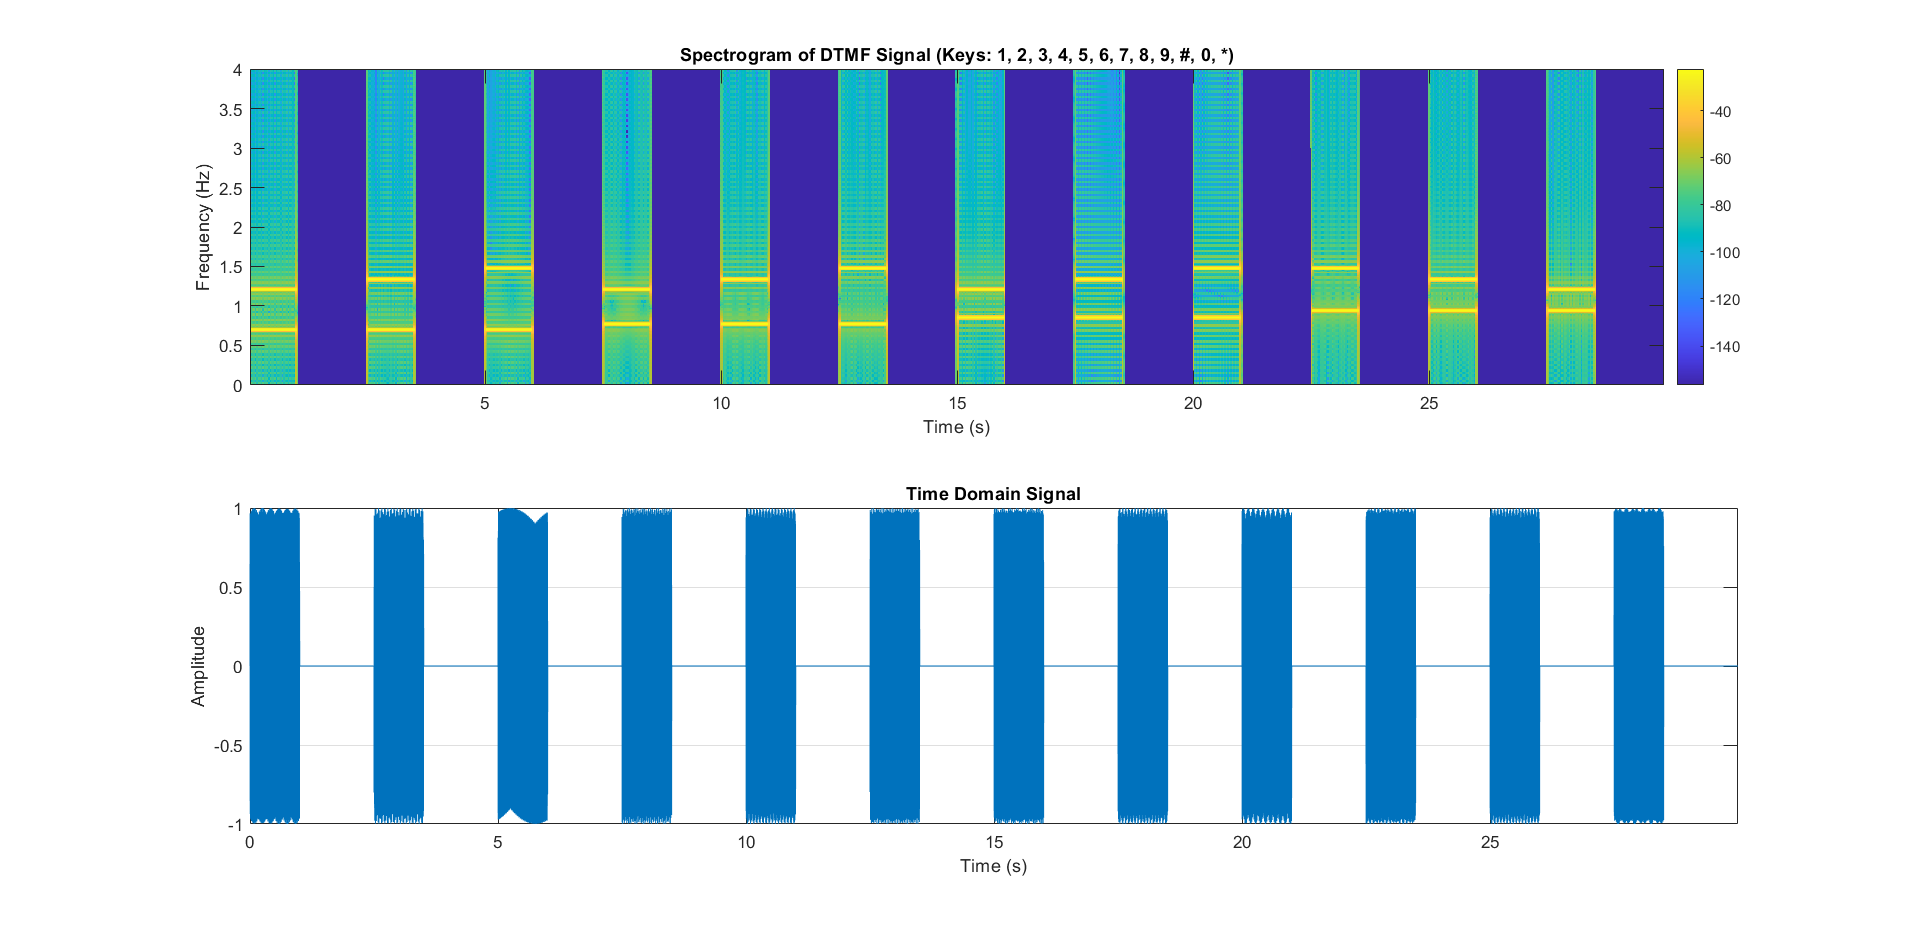
\includegraphics[width=0.8\linewidth]{dtmf.png}
%     \caption{DTMF signal in the time domain and its spectogram.}
%     \label{fig:dtmf_time}
% \end{figure}


\begin{figure}[h!]
    \centering
    \includegraphics[width=0.8\linewidth]{3.jpg}
    \caption{Power spectral density of the demodulated left audio signal (L) from the FM broadcast.}
    \label{fig:L_psd}
\end{figure}

\begin{figure}[h!]
    \centering
    \includegraphics[width=0.8\linewidth]{4.jpg}
    \caption{Power spectral density of the demodulated right audio signal (R) from the FM broadcast.}
    \label{fig:R_psd}
\end{figure}
\subsection*{Extracting the RDS Signal}

In this section, we extract the Radio Data System (RDS) signal from the demodulated FM baseband signal. RDS is a digital subcarrier typically transmitted at 57 kHz, which carries metadata such as station identification, song titles, or traffic information.

To isolate the RDS signal, we applied a narrow bandpass filter centered around 57 kHz using a FIR filter designed with the equiripple method. The filter had a passband from 56 to 58 kHz, effectively attenuating other frequency components while preserving the RDS content.

After filtering, the signal was processed to extract the encoded data. We first computed the instantaneous phase of the filtered signal using the \texttt{angle()} function. By unwrapping and differentiating this phase, we obtained the differential phase shifts corresponding to the RDS digital modulation. These phase differences were then thresholded to recover the binary DPSK (Differential Phase Shift Keying) symbols.

To decode the RDS bitstream, Manchester decoding was performed. The recovered bitstream was reshaped into symbol pairs, and each pair was interpreted based on standard Manchester coding rules (i.e., a transition from low to high represents a '1', while high to low represents a '0').

This decoded binary sequence contains the raw RDS data, which can be further parsed to extract useful information such as Program Identification (PI), Program Service (PS), or RadioText (RT), though full protocol decoding was beyond the scope of this session.

\begin{lstlisting}
%% step 10 -- getting the RDS signal --

bp_cutoff1 = 5.6e4; % Lower passband frequency in Hz
bp_cutoff2 = 5.8e4; % Upper passband frequency in Hz

%bpFilt2 = designfilt('bandpassfir', ...
%    'PassbandFrequency1', bp_cutoff1, ...
%    'StopbandFrequency1', (bp_cutoff1- 1e3), ...
%    'PassbandFrequency2', bp_cutoff2, ...
%    'StopbandFrequency2', (bp_cutoff2 + 1e3), ...
%    'SampleRate', fs, ...
%    'DesignMethod', 'equiripple');
load('bpFilt2.mat', 'bpFilt2');

%% step 11 -- getting the RDS signal & decoding it
filteredSignal5 = filter(bpFilt2, demodulated);
phase = angle(filteredSignal5);                       
dphase = diff(unwrap(phase));           
dpsk_bits = dphase > 0;  
manchester = 2*dpsk_bits - 1;
% Group into pairs
manchester_pairs = reshape(manchester, 2, []);
% Check transitions: (assuming IEEE 802.3: 1=LOW->HIGH, 0=HIGH->LOW)
decoded_bits = manchester_pairs(2,:) > manchester_pairs(1,:);


%%
% Step 1: Bandpass filter the 57 kHz subcarrier
filteredSignal5 = filter(bpFilt2, demodulated);

% Step 2: Downsample near 1187.5 Hz
target_bitrate = 1187.5;
decimation_factor_rds = round(fs / (2 * target_bitrate));  % 2 samples per bit
rds_signal = decimate(filteredSignal5, decimation_factor_rds);

% Step 3: BPSK demodulation
bpsk_bits = real(rds_signal) > 0;

% Step 4: Manchester decode from 2 samples per bit
% (e.g., HIGH->LOW = 0, LOW->HIGH = 1)
manchester_pairs = reshape(bpsk_bits(1:2*floor(end/2)), 2, []);
decoded_bits = manchester_pairs(2,:) > manchester_pairs(1,:);

\end{lstlisting}

\section*{Conclusion}
In this lab, we implemented a complete FM radio demodulation pipeline using MATLAB and real-world signals captured via the RTL-SDR USB dongle. Starting from the raw complex baseband signal, we applied appropriate filtering and demodulation techniques to extract the mono (L+R) audio signal, the stereo difference (L−R) signal, and finally reconstructed the left and right stereo channels. Additionally, we isolated and decoded the Radio Data System (RDS) subcarrier, demonstrating the ability to recover digital information embedded within the FM broadcast.

\end{document}
